%!TEX root = ../../../report.tex
\section{Robot creation} % (fold)
\label{sec:robot_creation}
One of the goals of the framework is to easy its continuity, thus this section is dedicated to explain how the robot was created.

A robot is defined as a set of links jointed.
A link contains at least three blocks of information:
\begin{enumerate}
   \item The collision model, used to calculate the collisions with other agents in the simulation.
   \item The visual model, uniquely used for visual purposes.
   \item The inertial information, that defines physical properties like the mass and the moments of inertia of the link.
\end{enumerate} 

A trade-off must be found for the precision of the collision model between accuracy and speed.
The more detailed is the model, the higher will be computation time which translates into more accuracy and more computation time.
The general advice is to have two simulation models: one for visual purposes and the other one for collisions.

In the case of the presented robot, the visual model is obtained directly exporting the parts from SolidWorks while the collision models is made of primitive gazebo shapes for the whole body but the feet.
Due to the robot is not meant to hit anything, the possible collisions in the body are not a priority, then each link is represented as a cylinder of the same length of the CAD model and a radius enough to cover the whole part.
An example can be seen in the figure \ref{fig:collision_model}.

The moments of inertia of each individual link are obtained directly from SolidWorks.
The CAD model includes the materials and thus the masses.
From these, the program is able to calculate the moments of inertia.
The figure \ref{fig:moments_of_inertia} shows the representation of these in the simulation.


\begin{figure}[hb!]
  \begin{subfigure}{.5\textwidth}
    \centering
    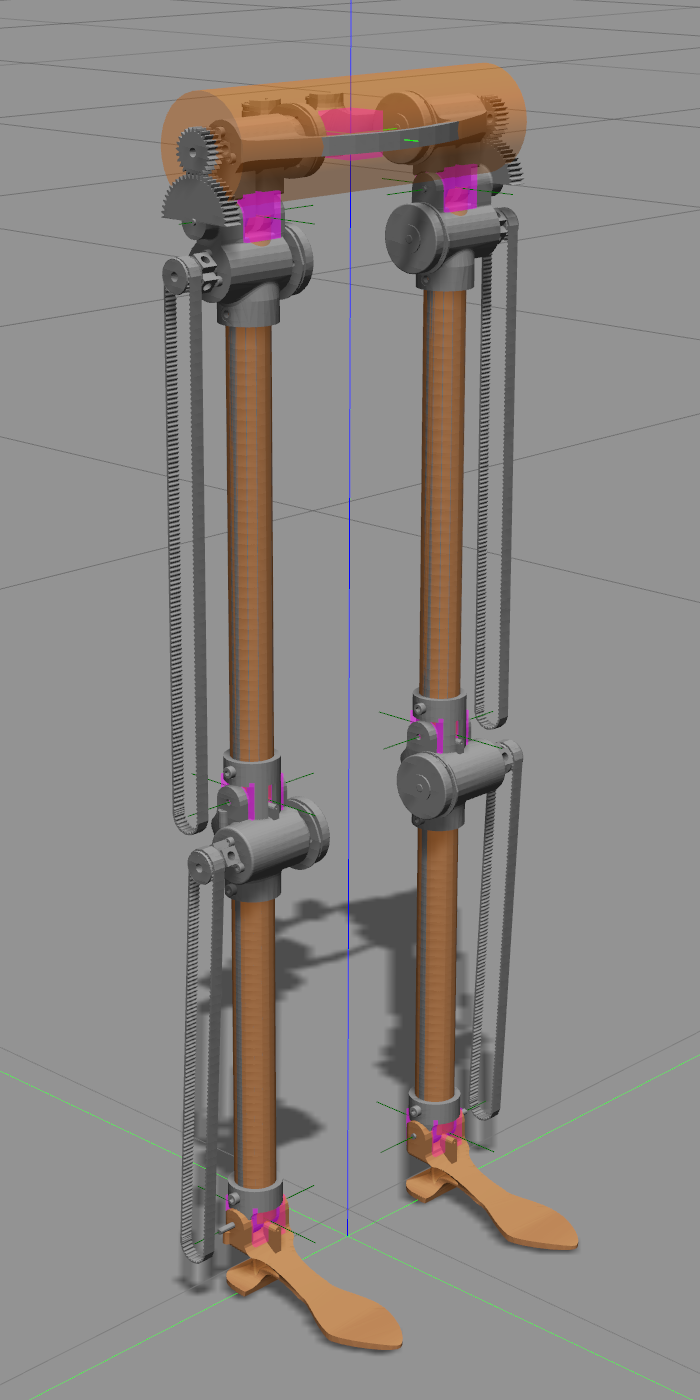
\includegraphics[width=.5\linewidth]{figures/gazebo_collision_model.png}
    \caption{Simulation in gazebo showing the visual model, the moments of inertia and the collision model}
    \label{fig:collision_model}
  \end{subfigure}%
  \begin{subfigure}{.5\textwidth}
    \centering
    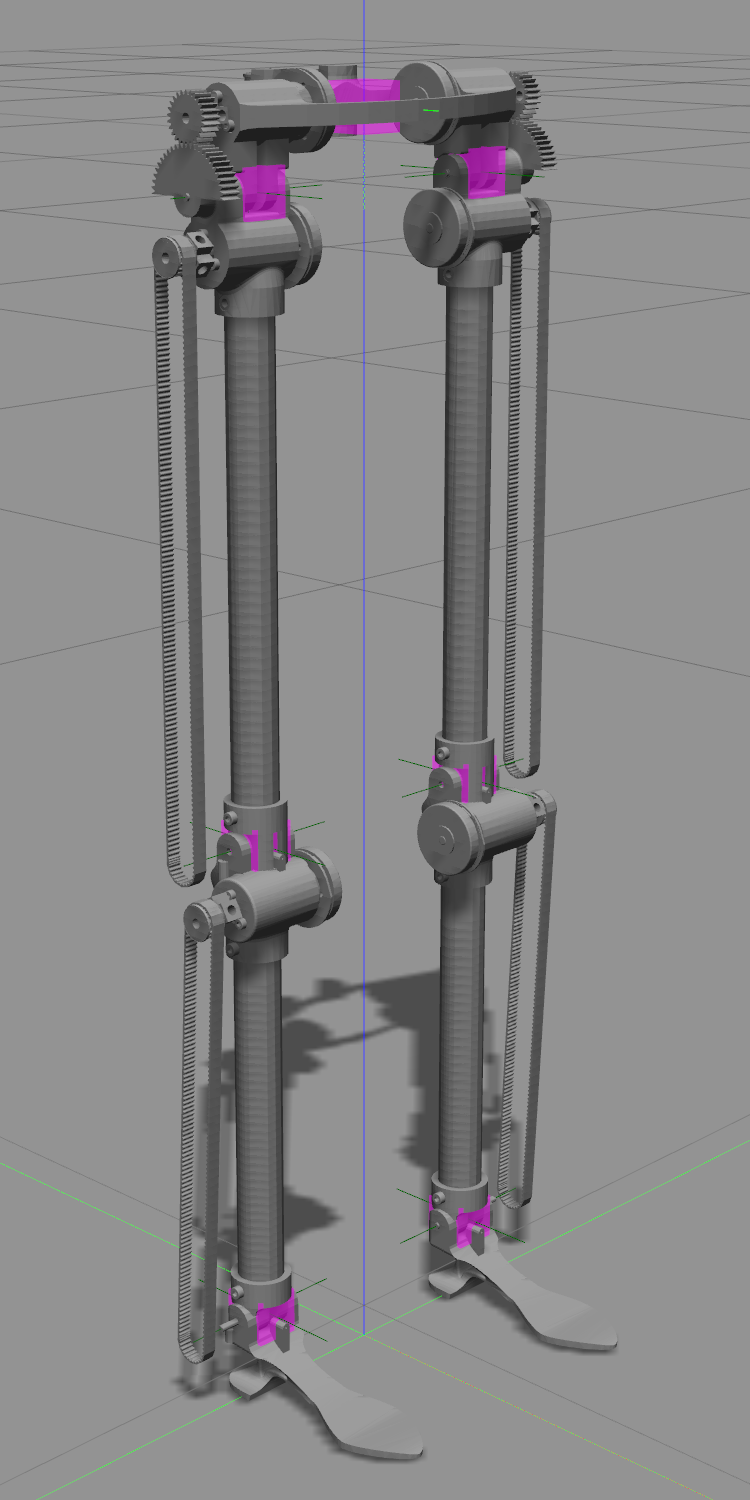
\includegraphics[width=.5\linewidth]{figures/gazebo_intertia_moments.png}
    \caption{LSimulation in gazebo showing the visual model and the moments of inertia}
    \label{fig:moments_of_inertia}
  \end{subfigure}
\end{figure}

It is important to notice that the visual models and moments of inertia have been exported from the correct reference frame.
In the case of the ankle, for example, the STL file and the moments of inertia are calculated from the reference frame positioned in the middle of the rotational axis of the ankle, pointing the Z axis to the rotational axis and Y to the biggest extension of the part.
This can be seen in the figure PUT THE FUCKING FIGURE FROM SOLIDWORKS HERE JORGE.

Finally, in the Xacro file the information that lacks the URDF and that must be added in Gazebo, have to be put.
In this file information as colors for the links can be added.
Eventually this description contains:
\begin{enumerate}
  \item \textbf{Plug-in for ROS Control}: Offers an interface for using ROS Control inside Gazebo.
  \item \textbf{Contact sensors}: Simulates contact sensors as in feet of the real robot.
  \item \textbf{Defines friction of the components}: as the friction between the feet and the floor.
\end{enumerate}

% section robot_creation (end)